1. Explain finite difference methods.
2. Derive the numerical methods and their truncation error (show error behaviour).

Methods included:
1. One-step method
    a. Euler's explicit
    b. Euler's implicit
    c. 4-stage Runge-Kutta method
    d. trapezium rule
    remarks: fixed point iteration method included to compute implicit methods
2. Predictor-corrector method
    a. Euler-trapezium method
3. Adaptive method
    a. ode23 method (Matlab)
    b. ode45 method (Matlab)
    
%---------------------------------------------------------------------------------
\chapter{Numerical methods}
\label{chap:numerical-methods}
%---------------------------------------------------------------------------------
In real world problems, ODE systems are frequently used. However, these models cannot be solved analytically. Therefore, the solution has to be estimated by numerical methods. The most popular and simple method is the Euler's method.

Intuitively, the Euler's explicit method tries to estimate the value at the next step following the gradient of the solution at current point. If the step size is sufficiently small, the estimation will be accurate.

An initial value problem, has the general form of 
\begin{align}
    y'&=f(x,y)\\
    y(x_0) &= y_0
\end{align}
for $x \in [x_0, X_M]$.

Notation:
Throughout the report, we will use the following notation.
$y_n$ - numerical approximation of $y(x_n)$
$y(x_n)$ - analytical solution at mesh point $x_n$
$x_n$ - mesh points of defined range, where

\begin{align}
    x_n &= x_0 + nh\\
    h &= \frac{(X_M - x_0)}{N}
\end{align}

for $n = 0,\dots, N$

For the simple Euler's explicit method, 
\begin{equation}
    y_{n+1} = y_n + hf(x_n,y_n)\\
\end{equation}

The implementation is as follows:

\begin{lstlisting}[language=Python]
y_n = [self.initial_value]
x_n = [self.x_min]

# Calculate approximated solution for each mesh point.
for n in range(1, self.mesh_points + 1):
    step = [self.mesh_size * f for f in self.func(x_n[-1], y_n[-1])]
    y_n.append([a + b for a, b in zip(y_n[-1], step)])
    x_n.append(self.x_min + n * self.mesh_size)

return x_n, y_n
\end{lstlisting}

inserting the analytical solution y(x) into the numerical method and dividing by the mesh
size is referred to as the consistency erro
The truncation error is obtained by the Taylor's expansion

The truncation error is defined to be the difference of exact solution with the numerical solution given the exact solution of previous mesh point is known. Therefore, we have that the truncation error for Euler's explicti method to be

\begin{equation}
    T_n \defeq \frac{y(x_{n+1}) - y(x_{n})}{h} - f(x_n, y(x_n))
\end{equation}

According to Taylor's series expansion, we have 
\begin{equation}
    y(x_n + h) = y(x_n) + hy'(x_n) + \frac{1}{2}h^2y''(\xi_n)
\end{equation}
for $\xi_n \in (x_n, x_{n+1})$. Substitute this to the truncation error, we get
\begin{equation}
    T_n = \frac{1}{2}h^2y''(\xi_n)
\end{equation}

Therefore, the truncation error for Euler's explicit method varies linearly with the step size.

In this report, we will use an example model $y'(x) = f(x,y) = -y$ to show that the implementation follow the theory.

Some examples of the solution to the given model can be found here: \href{https://nbviewer.jupyter.org/github/FarmHJ/numerical-solver/blob/issue-11-fhn-notebook/examples/solver_convergence.ipynb}{\hl{Example model notebook}}

Result image extracted from the notebook above shows that the truncation error follows 

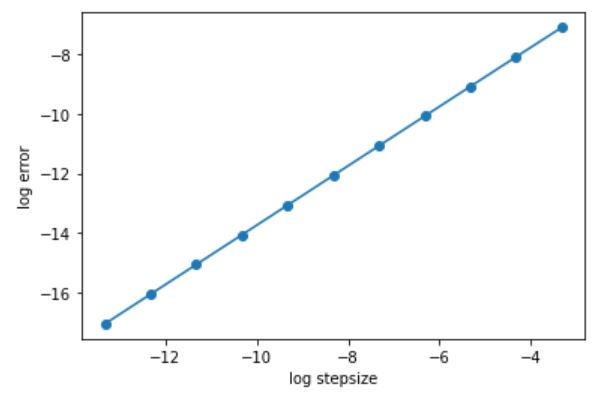
\includegraphics{Euler_explicit_error_behaviour}